Для демонстрации примерной работы приложения приведен пример внедрения трехмерной модели в веб-пространство. На \ref{figure:outro:3d} продемонстрирована перспективное окно проекции 
и набор инструментов для работы с трехмерной моделью.

\begin{figure}[ht]
    \centering
      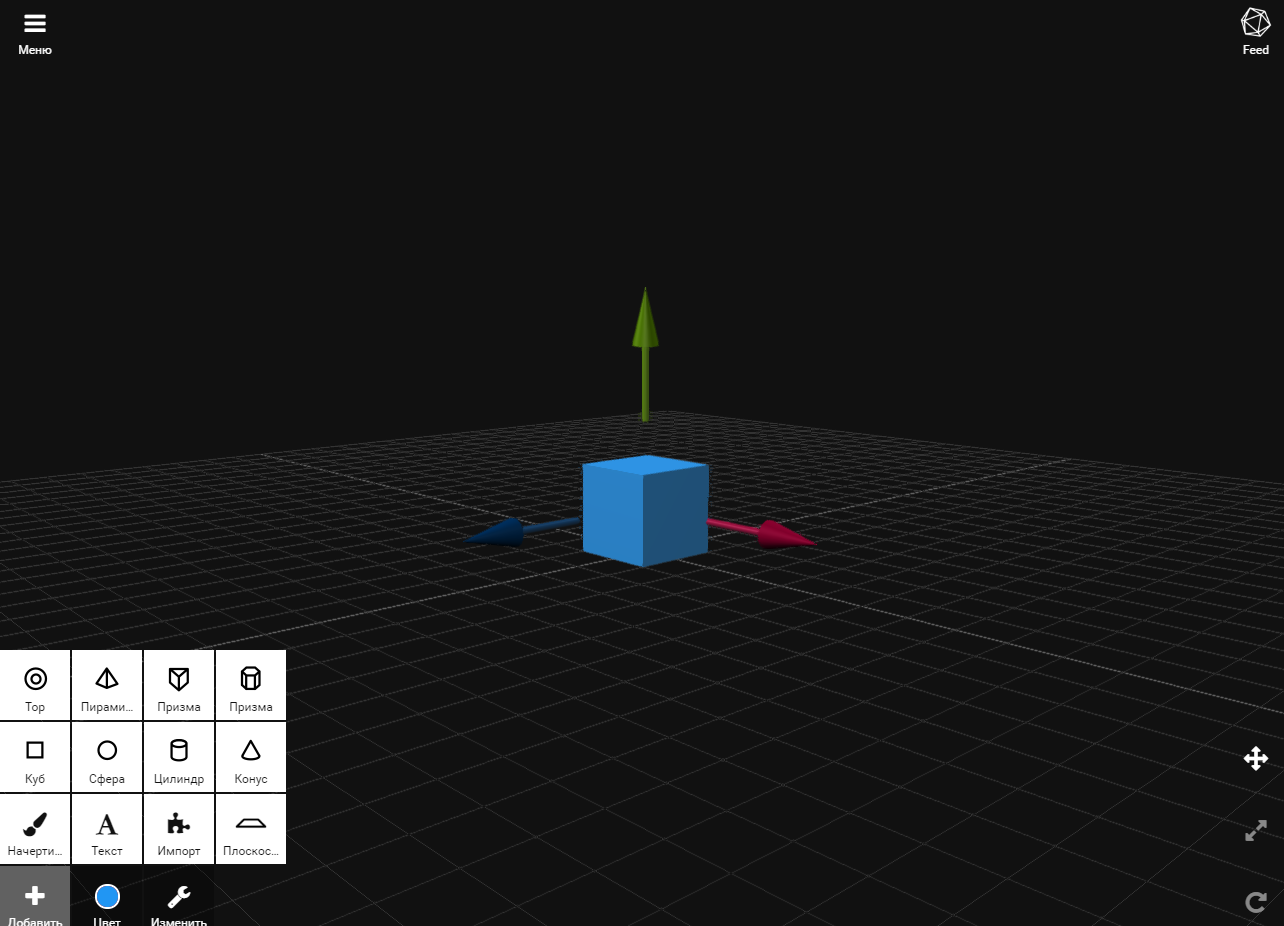
\includegraphics[scale=0.45]{outro-3d.png}
      \caption{Пример рабочей области для трехмерного моделирования в браузере}
      \label{figure:outro:3d}
\end{figure}
 
В данном веб-приложении предоставлена коллекция начальных трехмерных моделей и реализован минимальный набор функций для работы с ними. Реализованы 
такие функции как: Extrude, Group, Copy, Move, Delete. В результате настройки различных фильтров и несложных манипуляций в приложении будет возможно создать необходимую пользователю модель.

\begin{figure}[ht]
    \centering
      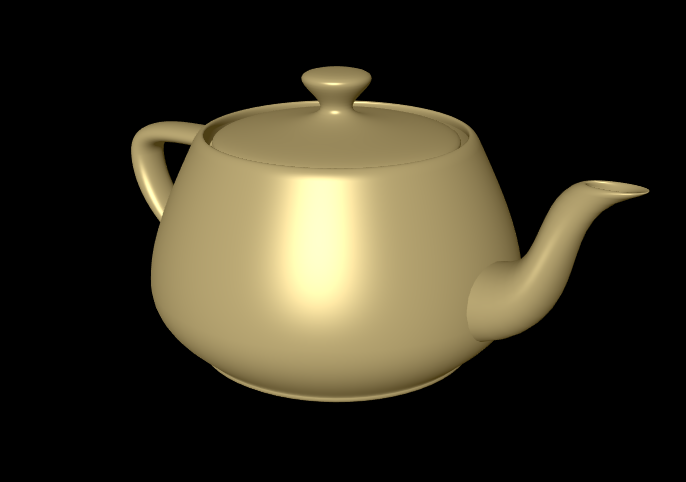
\includegraphics[scale=0.8]{teapot.png}
      \caption{Пример рабочей области для трехмерного моделирования в браузере}
      \label{figure:outro:3d}
\end{figure}